\documentclass[11pt]{article}

\usepackage{graphicx}
\usepackage{booktabs}
\usepackage{hyperref}
\usepackage{amsmath}
\usepackage{float}

\title{Inferring Container Workload Behavior from Host-Observable Telemetry}
\author{Anuj Lall}
\date{}

\begin{document}

\maketitle

\begin{abstract}
Modern container platforms expose coarse operational telemetry to the host system for monitoring and resource management. Even when containers are strongly isolated and the host cannot inspect container filesystems, memory, or internal execution, the host can still observe aggregate signals such as runtime, CPU usage, memory consumption, and disk I/O. This work investigates whether such host-observable telemetry alone can reveal information about containerized workloads.

We conduct a controlled measurement study on a Debian host running Docker containers under fixed resource limits. Three experiments are performed. First, we evaluate whether coarse telemetry can distinguish between several classes of workloads (CPU-bound, memory-bound, disk I/O-bound, and mixed). Using a simple Logistic Regression classifier trained on telemetry features, workload type can be predicted with 100\% accuracy in our experimental environment. Second, we examine whether telemetry signals can reveal a hidden parameter within a single workload. In a compression-based experiment where a secret parameter controls the entropy of input data, telemetry features enable prediction of the hidden parameter with 76\% accuracy, significantly above the random baseline.

Finally, we evaluate a simple mitigation based on output padding and runtime equalization designed to reduce observable differences between secret levels. While stronger padding reduces inference accuracy, it introduces substantial runtime overhead, illustrating a tradeoff between leakage reduction and performance cost.

Although the experiments are conducted in a simplified single-host environment, the results demonstrate that coarse container telemetry can contain information correlated with internal workload behavior. These findings highlight the importance of considering potential information leakage when exposing operational telemetry in containerized systems.
\end{abstract}

\section{Introduction}

Containerization is widely used to isolate applications while allowing a host system to manage and monitor resource usage. Even when strong isolation mechanisms prevent direct inspection of container contents, the host operating system typically retains access to coarse operational telemetry such as CPU usage, memory consumption, runtime, and disk I/O statistics. These signals are routinely collected for scheduling, monitoring, and debugging purposes. However, the extent to which such coarse host-observable telemetry may reveal information about containerized workloads is not always well understood.

This paper presents a small measurement study investigating whether standard host-visible telemetry from Docker containers is sufficient to reveal properties of the workload running inside the container. The study focuses on three progressively stronger questions. First, we ask whether basic telemetry features can distinguish between different classes of containerized workloads. Second, we examine whether the same signals can reveal a hidden parameter within a single workload. Finally, we evaluate whether a simple mitigation strategy can reduce this information leakage and quantify the associated performance overhead.

Our goal is not to demonstrate a sophisticated attack but rather to empirically measure how much information is exposed through coarse telemetry alone under a constrained threat model. All experiments are conducted on a single Debian host running Docker containers with fixed resource limits. The host is assumed to be an honest-but-curious operator who can observe standard container telemetry but cannot inspect container filesystems, memory, code, or network traffic.

Within this controlled environment, we conduct three experiments. The first experiment trains a classifier to distinguish among CPU-bound, memory-bound, disk I/O-bound, and mixed workloads using only host-observable telemetry features. The second experiment focuses on a single workload whose internal parameter controls data entropy and compressibility; we test whether telemetry signals can be used to infer this hidden parameter. The third experiment introduces a simple mitigation based on output padding and runtime equalization and evaluates how effectively it reduces the ability to infer the secret parameter while measuring the associated overhead.

The results of these experiments provide an empirical look at how much information may be exposed through coarse container telemetry in a simplified environment. While the study does not claim broad real-world exploitability, it illustrates how even limited host-visible signals can contain information about container behavior and highlights the tradeoff between reducing leakage and incurring performance overhead.

\section{Threat Model}

This study assumes an honest-but-curious host operator as the adversary. The attacker controls or operates the Linux host system on which containers are executed but does not actively interfere with the execution of the containers. Their goal is to infer information about the workloads running inside containers using only telemetry that is normally available to the host operating system.

The attacker is assumed to have access to standard host-level telemetry for Docker containers. In particular, the attacker can observe coarse resource usage metrics such as total runtime, CPU utilization, memory consumption, and block device I/O statistics. These signals are available through normal container monitoring mechanisms such as cgroup accounting and standard Docker runtime statistics. Importantly, the attacker observes only aggregate measurements for the container as a whole rather than detailed internal behavior.

Several capabilities are explicitly excluded from the attacker model. The attacker cannot inspect container filesystems, examine container code, or view the inputs provided to the containerized workloads. They also cannot access process memory, attach debuggers, or perform any form of syscall tracing. More advanced observability mechanisms such as eBPF instrumentation, kernel tracing frameworks, or performance counters are not available to the attacker.

Additionally, the attacker does not observe network traffic, does not instrument the kernel, and does not have visibility into internal container execution beyond the coarse telemetry exposed by the host. The experiments also assume a single-host environment without co-tenant interference, meaning that there are no other competing workloads generating noise in the system.

Under this threat model, the attacker’s task is purely observational: given a set of host-observable telemetry measurements for container runs, they attempt to infer properties of the workload running inside the container. The experiments in this paper evaluate how much information can be extracted under these constraints and how mitigation strategies affect this leakage.

\section{Experimental Setup}

All experiments are conducted on a single Debian Linux virtual machine that serves as the host operating system for the study. Containerized workloads are executed using Docker, with no additional sandboxing layers such as Kubernetes, gVisor, or microVM-based isolation. This simplified environment allows the experiments to focus specifically on the information exposed through standard container resource accounting mechanisms.

Each workload is executed inside a Docker container with fixed resource limits to ensure consistent execution conditions across runs. Containers are launched with a CPU limit of \texttt{--cpus=1} and a memory limit of \texttt{--memory=512m}. Network access is disabled when possible using \texttt{--network none}, or otherwise kept fixed and consistent across runs. These limits help reduce variability in resource availability and make telemetry measurements more comparable across experiments.

The host collects coarse container telemetry using standard cgroup accounting statistics exposed by the Docker runtime. For each container execution, a single row is recorded in a dataset capturing the following measurements:

\begin{itemize}
    \item \texttt{runtime\_ms}: total wall-clock execution time of the container run
    \item \texttt{avg\_cpu\_percent}: average CPU utilization derived from CPU usage counters and runtime
    \item \texttt{max\_mem\_mib}: peak container memory usage measured via \texttt{memory.current}
    \item \texttt{blk\_read\_mib}: total block device read volume
    \item \texttt{blk\_write\_mib}: total block device write volume
    \item \texttt{exit\_code}: container exit status
\end{itemize}

In addition to telemetry measurements, each dataset row includes experiment metadata used for analysis and labeling:

\begin{itemize}
    \item workload type
    \item workload intensity level
    \item workload parameter \texttt{N} (when applicable)
    \item repetition index (\texttt{rep})
    \item run identifier (\texttt{run\_id})
\end{itemize}

Some measurements require careful interpretation. For example, cgroup memory usage includes page cache, which means disk-heavy workloads may appear to use substantial memory due to caching effects. Similarly, block read activity may be underreported because frequently accessed data can be served from the page cache rather than the disk. Block write statistics are generally more reliable because writes must eventually propagate to the storage layer.

All experiments follow a repeated-run measurement methodology, where each workload configuration is executed many times to build a dataset suitable for statistical analysis and simple machine learning classification. This dataset serves as the basis for the experiments described in the following sections.

\begin{table}[H]
\centering
\begin{tabular}{ll}
\toprule
Component & Description \\
\midrule
Host OS & Debian Linux VM \\
Container Runtime & Docker \\
CPU Limit & 1 core (\texttt{--cpus=1}) \\
Memory Limit & 512 MB (\texttt{--memory=512m}) \\
Telemetry Source & cgroup statistics \\
Runs Collected & 360 (baseline), 200 (secret), 360 (mitigation) \\
\bottomrule
\end{tabular}
\caption{Experimental environment summary}
\label{tab:env_summary}
\end{table}

\section{Methodology}

The study follows a measurement-driven experimental methodology designed to determine whether coarse host-visible telemetry signals contain information about container workloads. Each experiment consists of repeatedly executing containerized workloads, recording host-observable telemetry for each run, and analyzing the resulting dataset using simple classification techniques.

For every container execution, the host records a fixed set of telemetry features including runtime, CPU utilization, peak memory usage, and block device I/O statistics. These measurements are stored as rows in a CSV dataset along with metadata identifying the workload configuration and repetition index. Repeated executions are used to capture natural variability in scheduling, caching behavior, and system noise while still allowing statistical patterns to emerge across runs.

To evaluate whether telemetry signals reveal information about the workload, we use simple and interpretable machine learning models, specifically Logistic Regression with feature standardization. The goal is not to optimize predictive performance but to determine whether easily accessible telemetry signals contain enough structure to distinguish between workload behaviors. Using a simple model helps ensure that any predictive performance is attributable to the telemetry features themselves rather than complex modeling techniques.

Each experiment follows a similar analysis procedure. After collecting telemetry data, the dataset is split into training and evaluation portions. The classifier is trained to predict the relevant label for the experiment—either workload type or a hidden parameter—and performance is measured using overall classification accuracy and confusion matrices. In addition to classification metrics, the analysis includes feature distribution visualizations to help interpret which signals contribute most strongly to distinguishability between classes.

The experiments are structured to answer three progressively stronger questions. The first experiment examines whether telemetry can distinguish between different categories of workloads. The second experiment focuses on whether telemetry can reveal a hidden parameter within a single workload, representing a more subtle form of information leakage. The third experiment evaluates whether simple mitigation strategies, based on padding resource usage, can reduce this leakage and quantifies the associated performance cost.

Together, these experiments provide a structured way to measure how much information may be exposed through coarse container telemetry under the threat model defined earlier.

\section{Baseline Workload Classification}

The first experiment establishes a baseline by testing whether coarse host-observable telemetry is sufficient to distinguish between different classes of containerized workloads. The goal of this experiment is not to infer hidden information but rather to determine whether basic workload behavior can be identified using only the limited telemetry available to the host under the defined threat model.

Four representative workload types are implemented for this experiment:

\begin{itemize}
    \item \textbf{CPU-bound:} performs intensive computation with minimal memory allocation and little disk activity.
    \item \textbf{Memory-bound:} repeatedly allocates and accesses large memory buffers to stress memory usage.
    \item \textbf{Disk I/O-bound:} performs repeated disk write operations to generate sustained block device activity.
    \item \textbf{Mixed workload:} combines moderate CPU computation, memory access, and disk writes.
\end{itemize}

Each workload accepts a parameter \texttt{N} controlling workload intensity, allowing three levels of execution cost: low, medium, and high. This parameter changes the amount of computation, memory allocation, or I/O performed by the workload while keeping the overall workload type consistent. Varying intensity ensures that the classifier must identify workload type rather than relying solely on absolute runtime differences.

For each combination of workload type and intensity level, the workload is executed repeatedly inside a Docker container under the fixed resource limits described earlier. Approximately 30 repetitions are performed for each configuration. With four workload types and three intensity levels, this results in a dataset of roughly 360 container executions.

For every run, the host records telemetry features including runtime, CPU utilization, peak memory usage, and block device I/O statistics. These measurements form the feature vector used for classification. The ground-truth label for the experiment is the workload type.

To evaluate whether the telemetry signals contain distinguishable patterns, a Logistic Regression classifier with standardized features is trained to predict the workload type from the recorded telemetry. Performance is evaluated using classification accuracy and a confusion matrix, which indicates how frequently the classifier confuses one workload type for another. The baseline confusion matrix is shown in Figure~\ref{fig:baseline_cm}.

\begin{figure}[H]
\centering
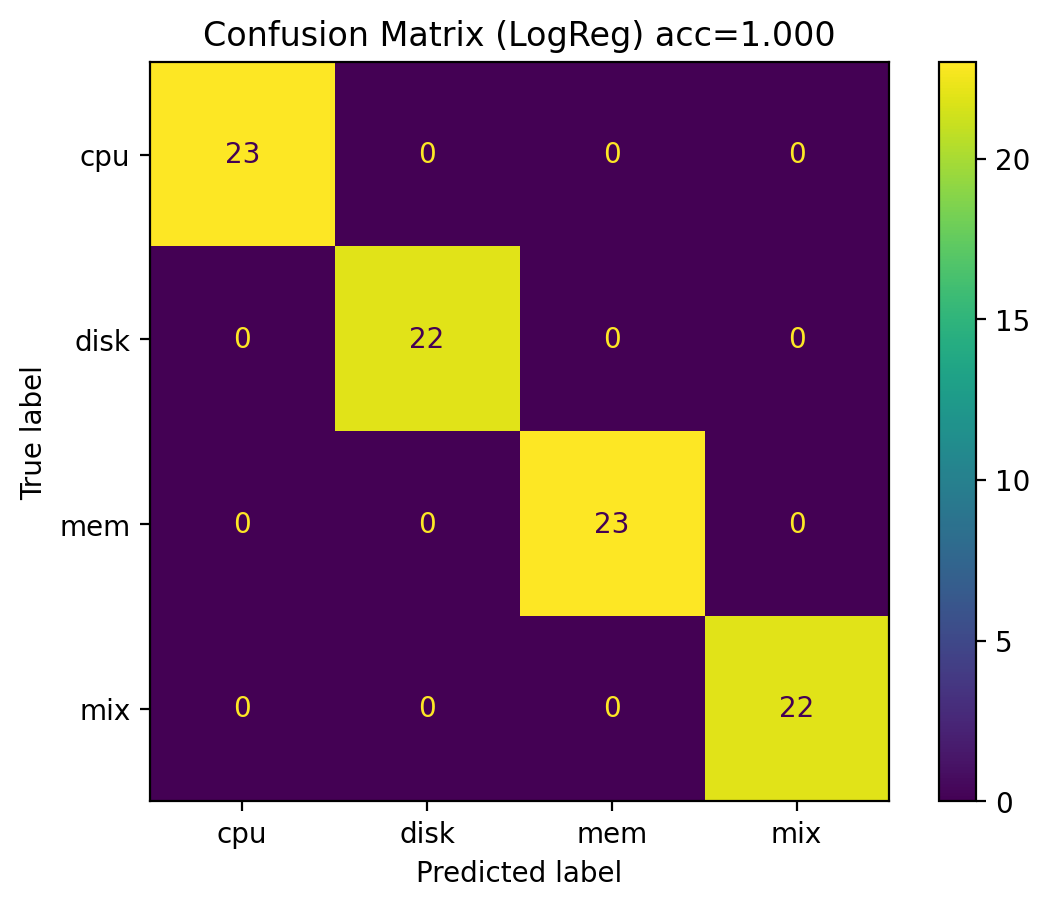
\includegraphics[width=0.7\linewidth]{figures/baseline_confusion_matrix.png}
\caption{Confusion matrix for baseline workload classification}
\label{fig:baseline_cm}
\end{figure}

In addition to classification metrics, we visualize the distribution of key telemetry signals across workloads. In particular, we examine runtime distributions by workload type and memory usage distributions by workload type. These plots, shown in Figure~\ref{fig:runtime_workload} and Figure~\ref{fig:mem_workload}, provide intuition about which signals contribute most strongly to distinguishing between workloads and help interpret the classification results.

\begin{figure}[H]
\centering
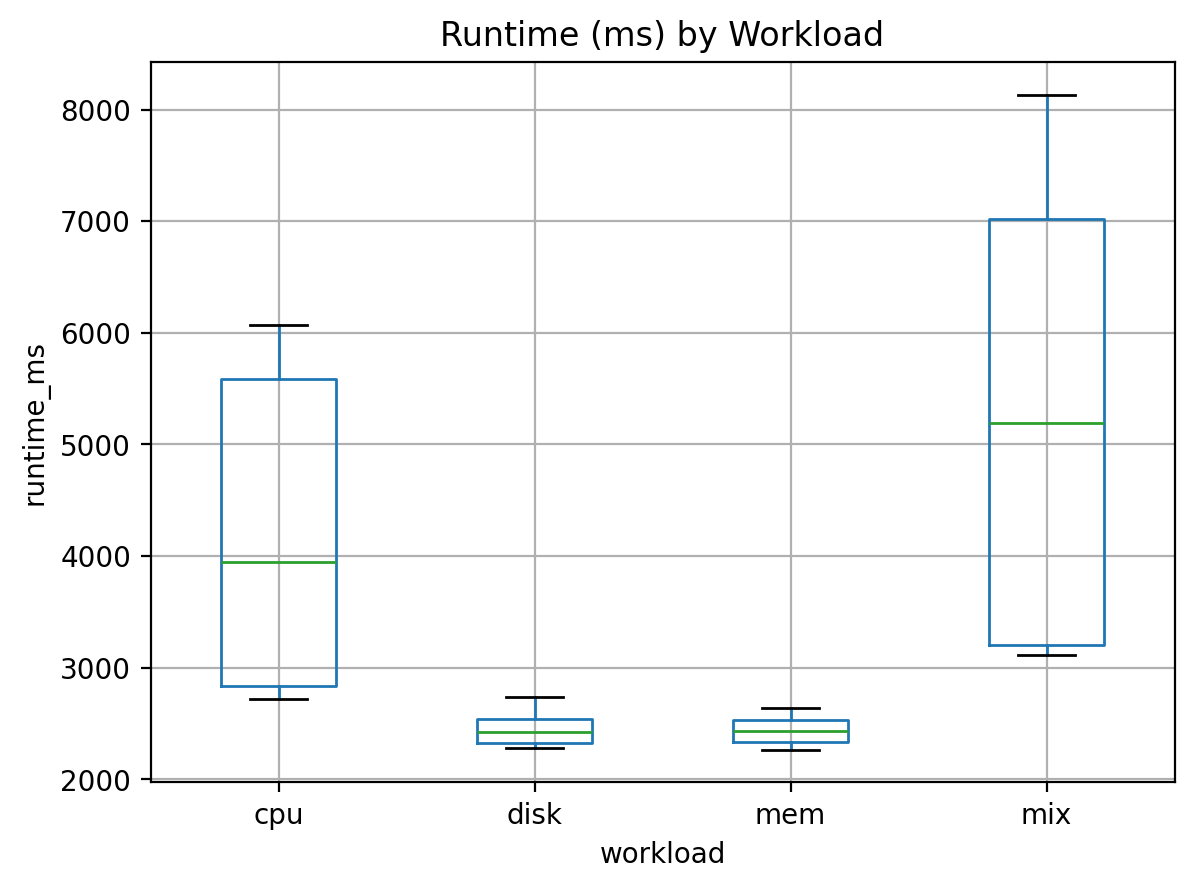
\includegraphics[width=0.7\linewidth]{figures/runtime_by_workload.png}
\caption{Runtime distribution by workload type}
\label{fig:runtime_workload}
\end{figure}

\begin{figure}[H]
\centering
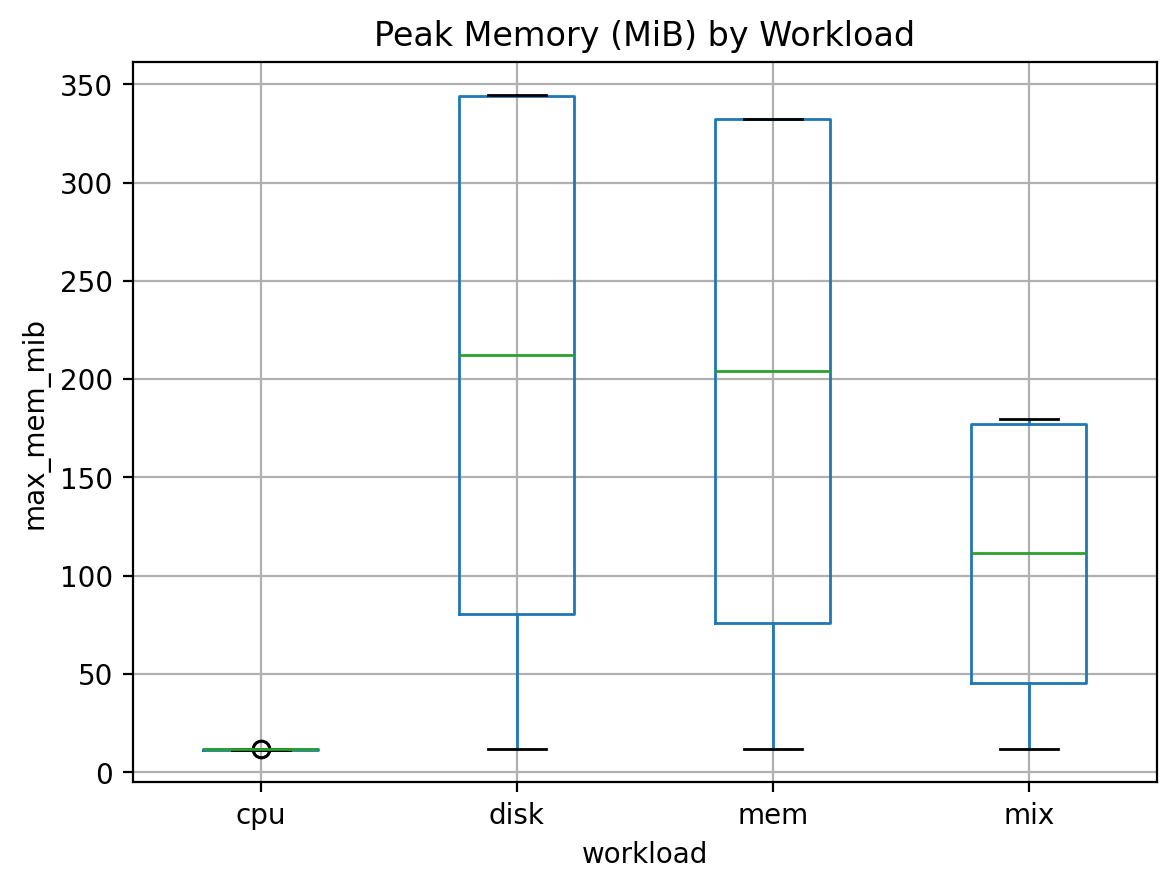
\includegraphics[width=0.7\linewidth]{figures/memory_by_workload.png}
\caption{Peak memory usage by workload type}
\label{fig:mem_workload}
\end{figure}

\section{Secret Parameter Inference}

The second experiment investigates a more subtle question: whether host-observable telemetry can reveal a hidden parameter within a single workload. Unlike the baseline experiment, where different workload types were intentionally distinct, this experiment focuses on a single program whose internal behavior changes based on a parameter that is not visible to the host.

The workload used in this experiment generates a fixed-size memory buffer and then compresses it using \texttt{gzip}. The size of the buffer remains constant across runs (e.g., \texttt{size\_mib = 128}), but the entropy of the data within the buffer is controlled by a hidden parameter called \texttt{secret\_N}. This parameter determines how compressible the data is before compression.

Four possible values of \texttt{secret\_N} are used:

\begin{itemize}
    \item \textbf{0 --- All zeros:} the buffer contains only zero bytes, making it highly compressible.
    \item \textbf{1 --- Repeating pattern:} the buffer contains a simple repeating sequence of bytes, which is also strongly compressible.
    \item \textbf{2 --- Small alphabet pseudo-random:} the buffer is generated from a limited character set, producing moderate entropy.
    \item \textbf{3 --- High-entropy random:} the buffer is filled using \texttt{os.urandom}, producing nearly incompressible data.
\end{itemize}

After generating the buffer, the workload compresses it in memory using \texttt{gzip} and writes the compressed output to disk. The program then forces the write to disk using \texttt{fsync} to ensure that the disk I/O is reflected in the host-observable telemetry. The container then exits normally.

Although the host cannot inspect the contents of the buffer or the compressed file, differences in compressibility affect observable system behavior. Highly compressible data produces much smaller output files and typically completes faster, while incompressible data results in larger disk writes and potentially longer execution times. These differences may appear in the telemetry signals available to the host.

The experiment protocol executes the workload repeatedly for each value of \texttt{secret\_N}. Approximately 50 repetitions per secret level are performed, resulting in a dataset of roughly 200 container runs. For each run, the host records the same telemetry features used in the baseline experiment: runtime, CPU usage, peak memory usage, and block device I/O statistics.

Using these features, a classifier is trained to predict the value of \texttt{secret\_N} from the telemetry alone. As before, we use a simple Logistic Regression model with standardized features. Performance is evaluated using classification accuracy and a confusion matrix to determine how reliably the hidden parameter can be inferred. The confusion matrix for this experiment is shown in Figure~\ref{fig:secret_cm}.

\begin{figure}[H]
\centering
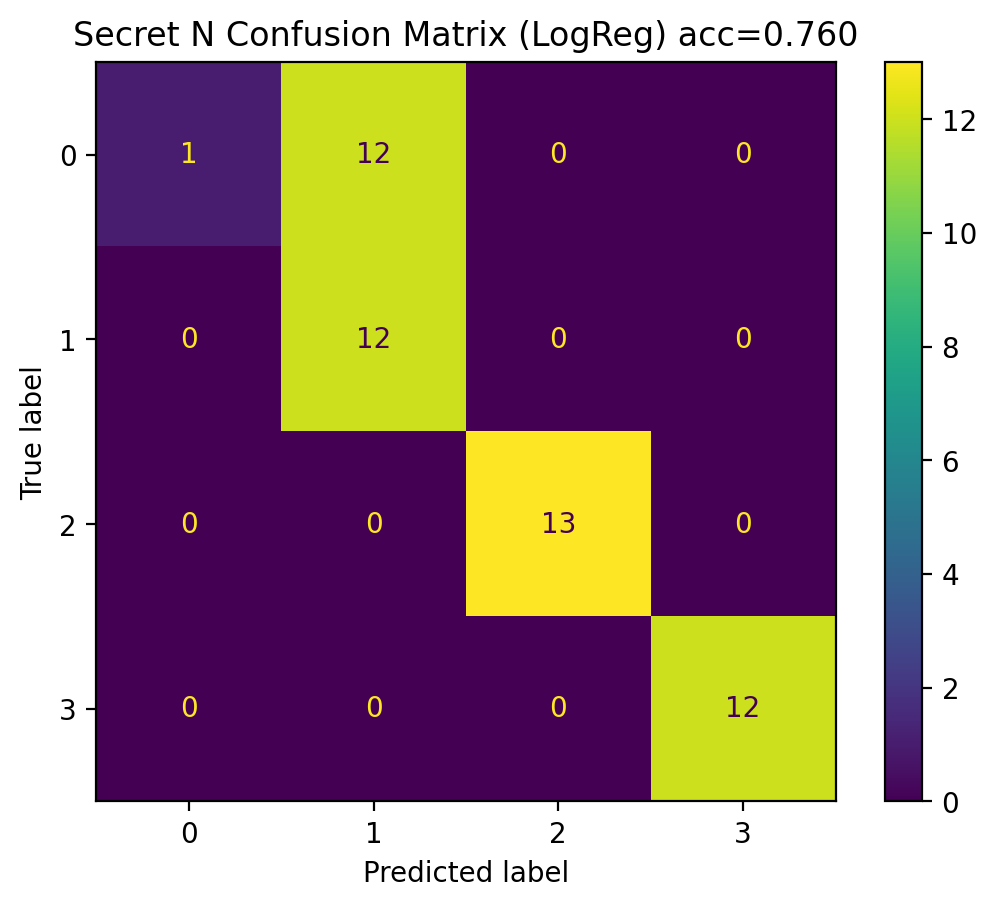
\includegraphics[width=0.7\linewidth]{figures/secret_confusion_matrix.png}
\caption{Confusion matrix for secret parameter inference}
\label{fig:secret_cm}
\end{figure}

To better understand the leakage mechanism, we also examine feature distributions across secret levels. In particular, we analyze block write volume (\texttt{blk\_write\_mib}) by \texttt{secret\_N} and runtime (\texttt{runtime\_ms}) by \texttt{secret\_N}. These plots, shown in Figure~\ref{fig:secret_write} and Figure~\ref{fig:secret_runtime}, help illustrate which host-observable signals are most strongly correlated with the hidden parameter and therefore most responsible for any successful inference.

\begin{figure}[H]
\centering
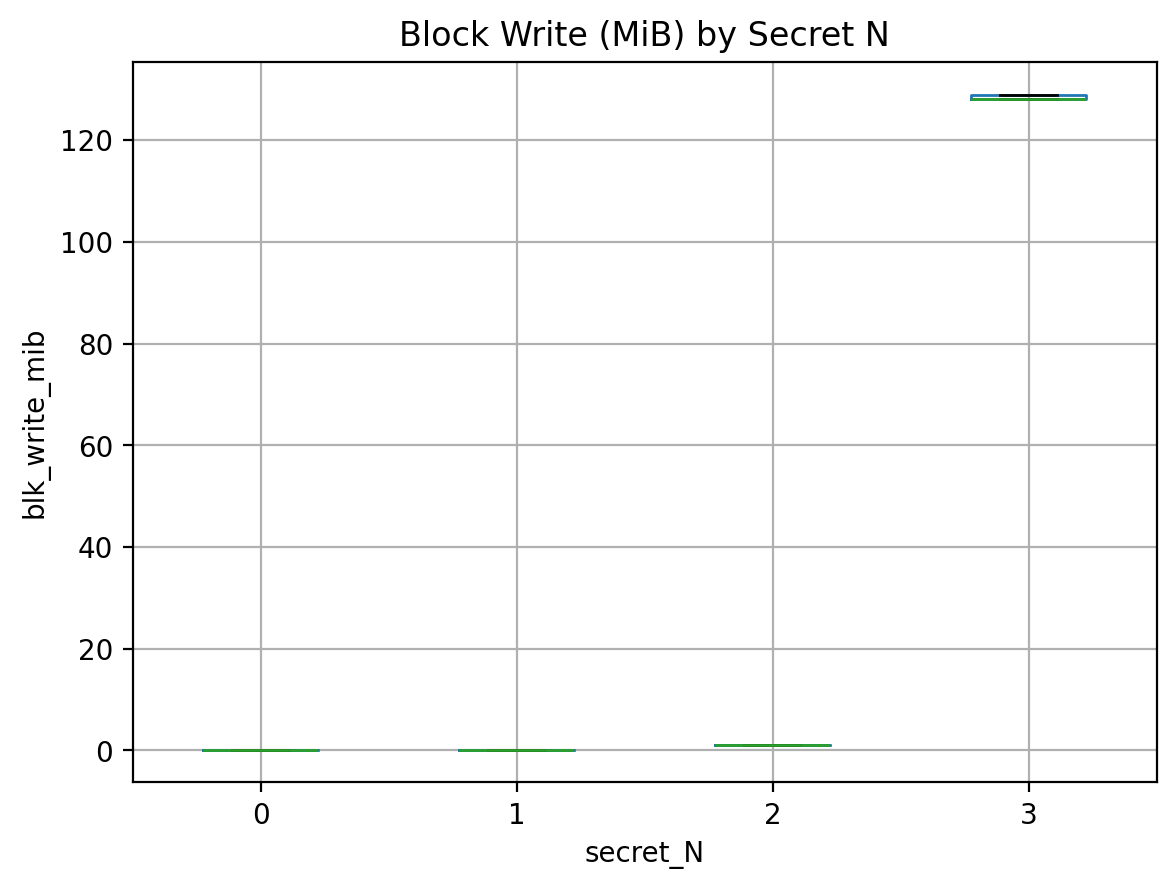
\includegraphics[width=0.7\linewidth]{figures/secret_blk_write.png}
\caption{Block write volume by secret level}
\label{fig:secret_write}
\end{figure}

\begin{figure}[H]
\centering
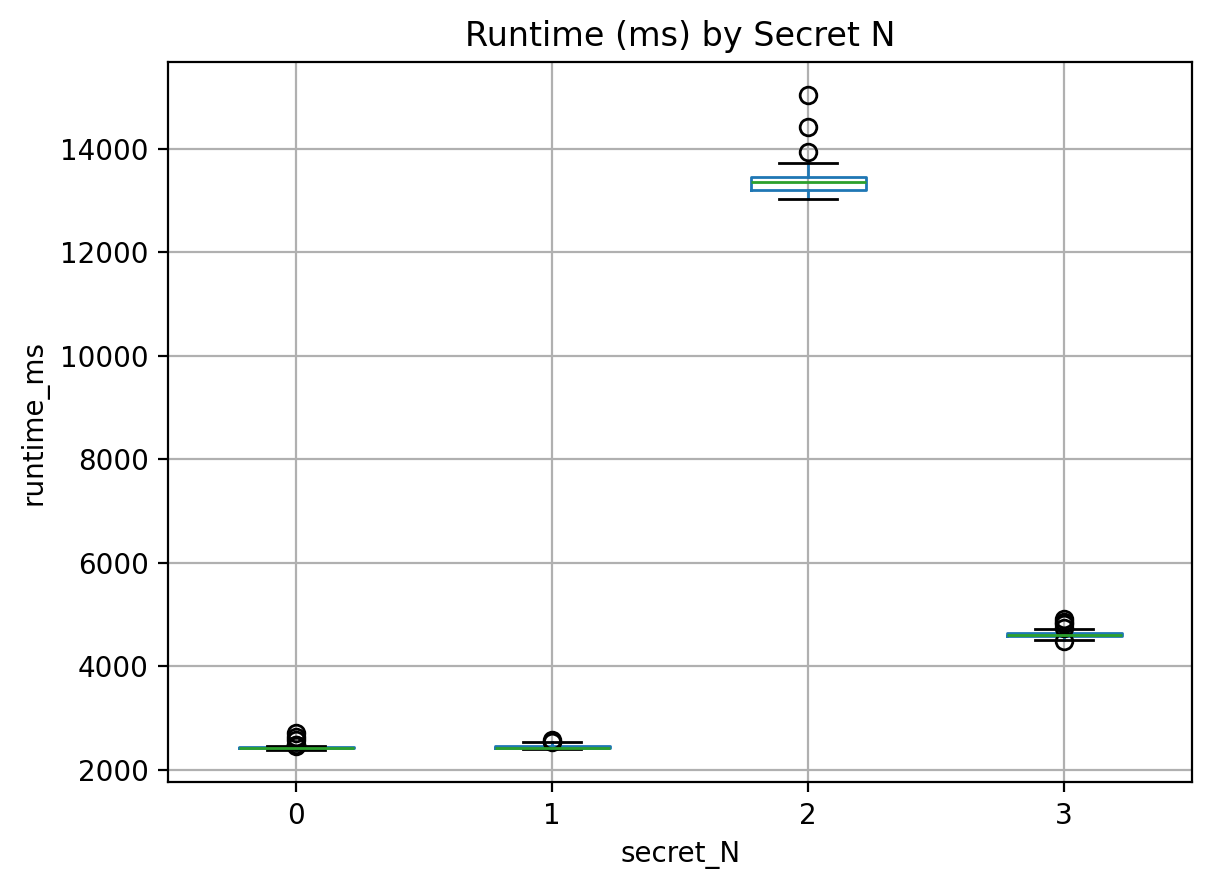
\includegraphics[width=0.7\linewidth]{figures/secret_runtime.png}
\caption{Runtime distribution by secret level}
\label{fig:secret_runtime}
\end{figure}

\section{Mitigation Evaluation}

The third experiment evaluates whether simple padding-based mitigations can reduce the ability to infer the hidden parameter observed in the previous experiment. The goal is not to eliminate leakage entirely but to measure how much inference accuracy can be reduced and what performance overhead is required to achieve that reduction.

The mitigation strategy focuses on neutralizing the two primary telemetry channels identified in the secret inference experiment: disk write volume and total runtime. Two forms of padding are therefore introduced: disk padding and time padding. These mechanisms intentionally make observable resource usage less dependent on the compressibility of the data.

\subsection*{Disk Padding (Output Size Equalization)}

After the compressed data is written to disk, the workload appends additional zero bytes until the output file reaches a predetermined target size. The target size depends on the mitigation strength:

\begin{itemize}
    \item \textbf{none:} no padding is applied; the compressed file is written as-is.
    \item \textbf{low:} the output file is padded up to 64 MiB if the compressed output is smaller than this threshold.
    \item \textbf{high:} the output file is padded up to 140 MiB, which is chosen to exceed the worst-case compressed size for the 128 MiB input buffer.
\end{itemize}

This padding mechanism attempts to reduce leakage through the \texttt{blk\_write\_mib} signal by forcing disk write volumes to converge toward a constant size.

\subsection*{Time Padding (Runtime Equalization)}

The second mitigation attempts to reduce leakage through execution time differences. After completing the actual workload, the program ensures that the total runtime reaches a minimum threshold. If the real computation finishes early, the container performs additional CPU work (e.g., hashing loops) until the minimum runtime is reached.

The runtime thresholds depend on the mitigation level:

\begin{itemize}
    \item \textbf{none:} no runtime equalization is applied.
    \item \textbf{low:} enforce a minimum total runtime of approximately 8 seconds.
    \item \textbf{high:} enforce a minimum total runtime of approximately 18 seconds, chosen to exceed the worst observed execution time without padding.
\end{itemize}

A short hold period (approximately 2000 ms) may also be used to keep the container alive long enough to ensure stable telemetry measurements.

\subsection*{Experimental Protocol}

To evaluate the effectiveness of these mitigations, the experiment varies both the secret parameter and the mitigation level:

\[
\texttt{secret\_N} \in \{0,1,2,3\}
\]
\[
\texttt{mitigation} \in \{\texttt{none}, \texttt{low}, \texttt{high}\}
\]

Each configuration is executed approximately 30 times, producing a dataset of roughly 360 runs.

For each mitigation level, the same telemetry features are collected and used to train a classifier predicting \texttt{secret\_N}. By comparing classification accuracy across mitigation settings, we can measure how much the padding strategies reduce the ability to infer the hidden parameter.

In addition to leakage reduction, the experiment also measures performance overhead. For each mitigation level, the median runtime is compared to the baseline (no mitigation) runtime to quantify the additional cost introduced by padding.

The results of this experiment therefore capture the tradeoff between leakage reduction and performance overhead, illustrating how stronger mitigation strategies may reduce inference accuracy while increasing execution time. The corresponding accuracy and overhead plots are shown in Figure~\ref{fig:mitigation_accuracy} and Figure~\ref{fig:mitigation_overhead}.

\begin{figure}[H]
\centering
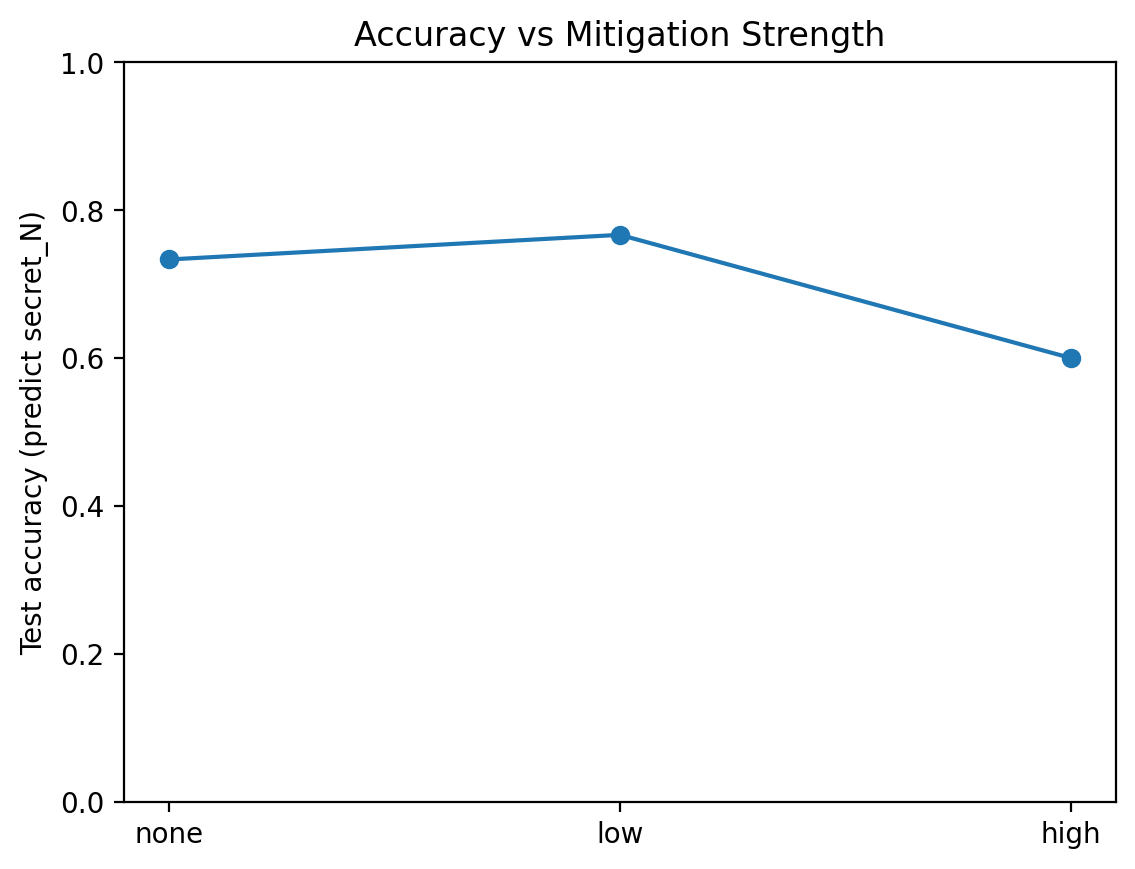
\includegraphics[width=0.7\linewidth]{figures/mitigation_accuracy.png}
\caption{Inference accuracy vs mitigation strength}
\label{fig:mitigation_accuracy}
\end{figure}

\begin{figure}[H]
\centering
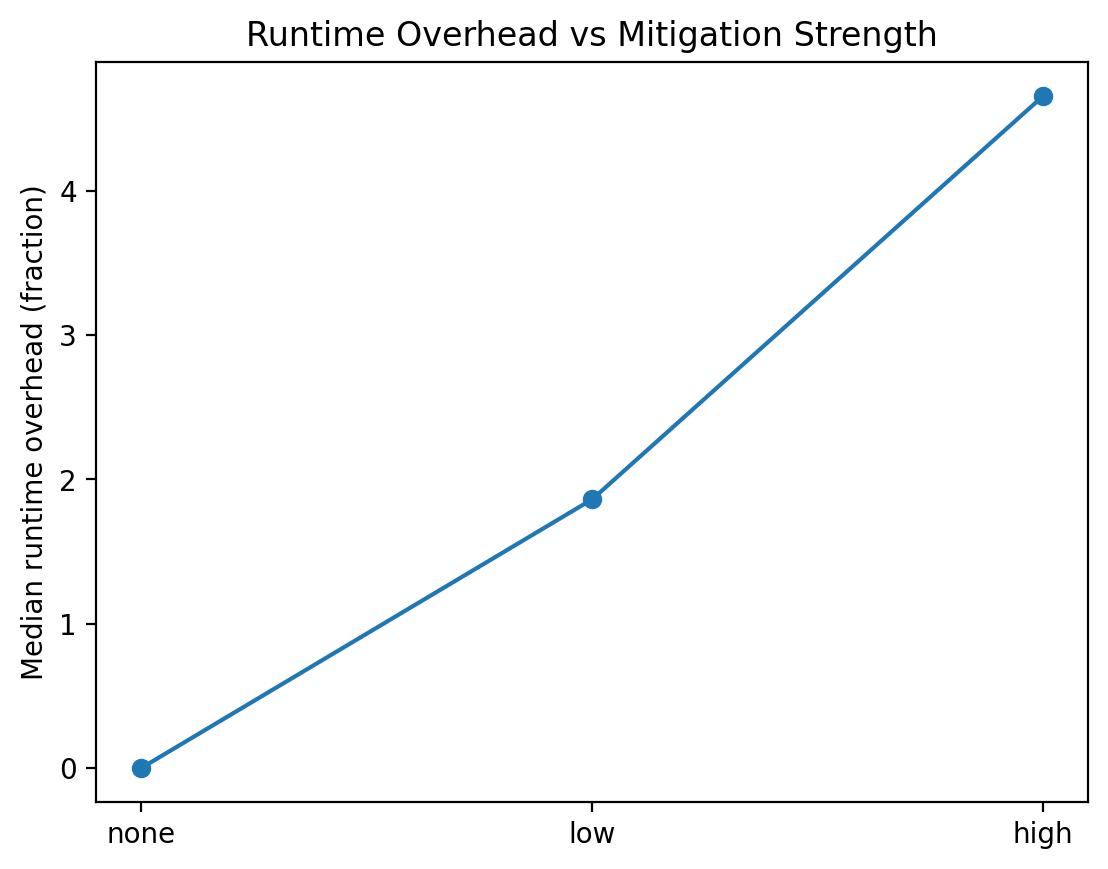
\includegraphics[width=0.7\linewidth]{figures/mitigation_overhead.png}
\caption{Runtime overhead vs mitigation strength}
\label{fig:mitigation_overhead}
\end{figure}

\section{Results}

This section presents the empirical results from the three experiments described earlier. The goal of these experiments is to evaluate how much information about container workloads can be inferred using only coarse host-observable telemetry under the defined threat model. Results are reported using classification accuracy, confusion matrices, and feature distribution plots to illustrate which signals contribute most strongly to inference.

\subsection{Baseline Workload Classification}

The first experiment evaluates whether host-level telemetry can distinguish between four workload types: CPU-bound, memory-bound, disk I/O-bound, and mixed workloads.

The dataset used for this experiment contains 360 container runs (all with successful exit codes). Each run is represented by the telemetry feature vector:

\begin{itemize}
    \item \texttt{runtime\_ms}
    \item \texttt{avg\_cpu\_percent}
    \item \texttt{max\_mem\_mib}
    \item \texttt{blk\_read\_mib}
    \item \texttt{blk\_write\_mib}
\end{itemize}

A Logistic Regression classifier with feature standardization is trained to predict the workload type.

The classifier achieves a test accuracy of 1.00, significantly above the random baseline of approximately 0.25 for a four-class classification problem.

The confusion matrix in Figure~\ref{fig:baseline_cm} shows perfect classification across all workload types, with no misclassifications between the four classes. This indicates that the telemetry signals provide strong separability between the workload behaviors in this experimental environment.

The distribution plots in Figure~\ref{fig:runtime_workload} and Figure~\ref{fig:mem_workload} further illustrate why this classification is possible. Runtime varies noticeably between workloads, particularly for the mixed workload which tends to run longer than the disk or memory workloads. Similarly, peak memory usage differs significantly across workload types. The memory-bound and disk workloads exhibit substantially higher peak memory usage than the CPU workload, largely due to page cache effects included in cgroup memory accounting.

These results demonstrate that coarse host-level telemetry is sufficient to reliably distinguish between broad categories of containerized workloads under the experimental conditions used in this study.

\subsection{Secret Parameter Inference}

The second experiment examines whether host-observable telemetry can reveal a hidden parameter within a single workload. In this experiment, the workload generates a fixed-size buffer and compresses it using \texttt{gzip}. The hidden parameter \texttt{secret\_N} controls the entropy of the input data, which directly affects compressibility.

The dataset for this experiment contains 200 container runs with four possible values of \texttt{secret\_N}. The same telemetry feature set used in the baseline experiment is used for classification.

A Logistic Regression classifier trained on these features achieves a test accuracy of 0.76, compared to the random baseline of approximately 0.25.

The confusion matrix in Figure~\ref{fig:secret_cm} shows that most secret levels are predicted correctly, though some confusion occurs between the lowest entropy levels. In particular, the classifier frequently predicts \texttt{secret\_N = 1} when the true label is \texttt{secret\_N = 0}, indicating that the telemetry signals for these two cases are similar.

Feature distribution plots in Figure~\ref{fig:secret_write} and Figure~\ref{fig:secret_runtime} reveal the underlying leakage mechanism. The block write volume (\texttt{blk\_write\_mib}) varies dramatically across secret levels. Highly compressible inputs produce extremely small compressed outputs, while high-entropy inputs produce compressed files close to the original buffer size. As a result, disk write volume becomes a strong observable signal correlated with the hidden parameter.

Runtime also varies across secret levels, particularly for the higher entropy inputs where compression work increases. This additional signal further helps the classifier distinguish between secret values.

Overall, these results show that host-observable telemetry can leak information about internal workload parameters, even when the host cannot inspect the container's contents or code.

\subsection{Mitigation Impact on Secret Inference}

The third experiment evaluates whether simple padding strategies can reduce the ability to infer the hidden parameter. The mitigation combines disk padding, which attempts to equalize output sizes, and time padding, which enforces a minimum runtime.

The experiment evaluates three mitigation levels: none, low, and high, each tested with the same classification procedure.

Prediction accuracy for the hidden parameter is:

\begin{itemize}
    \item \textbf{none:} 0.733
    \item \textbf{low:} 0.767
    \item \textbf{high:} 0.600
\end{itemize}

The strongest mitigation reduces inference accuracy to 0.60, which is still above the random baseline of 0.25 but represents a noticeable reduction compared to the unmitigated setting.

The runtime overhead introduced by the mitigation is substantial. Median container runtime increases from approximately 3.57 seconds with no mitigation to 10.23 seconds under the low mitigation and 20.22 seconds under the high mitigation. This corresponds to runtime overheads of approximately 1.86$\times$ and 4.66$\times$ relative to the baseline.

Figure~\ref{fig:mitigation_accuracy} and Figure~\ref{fig:mitigation_overhead} illustrate this tradeoff directly. Padding strategies can reduce the distinguishability of telemetry signals and thereby reduce leakage, but doing so introduces measurable performance overhead. Even with relatively strong padding, however, the telemetry signals remain partially informative, suggesting that completely eliminating leakage through simple padding alone may be difficult.

\section{Discussion and Limitations}

The results of this study illustrate that coarse host-observable telemetry can reveal meaningful information about container workloads, even when the host cannot inspect container contents or execution directly. In the baseline experiment, telemetry signals such as runtime and memory usage were sufficient to perfectly distinguish between several broad workload categories. In the second experiment, the same telemetry features enabled partial inference of a hidden parameter within a single workload, demonstrating that observable system behavior can correlate with internal data properties such as compressibility.

The mitigation experiment highlights an important leakage--performance tradeoff. Padding strategies that attempt to equalize disk write volume and execution time can reduce the ability of a classifier to infer the hidden parameter. However, achieving stronger mitigation requires substantial increases in runtime. Even with aggressive padding, inference accuracy remains above random chance, suggesting that eliminating leakage entirely may require more comprehensive approaches or stronger forms of isolation.

Several limitations should be considered when interpreting these results.

First, the experiments were conducted in a single-host environment without co-tenant interference. In real systems, additional workloads, background services, and scheduler variability may introduce noise that could either obscure or amplify telemetry-based inference signals. The simplified environment used here isolates the measurement problem but does not capture the full complexity of multi-tenant systems.

Second, the workloads used in this study are synthetic and intentionally structured to create observable differences in resource usage. While this approach allows the leakage mechanisms to be studied clearly, real-world applications may exhibit more complex behavior that is harder to classify using simple telemetry features.

Third, the attacker model assumes access only to coarse cgroup-based telemetry. Many real-world monitoring systems expose richer signals such as detailed performance counters, syscall traces, or kernel-level instrumentation. Access to these signals could potentially increase the strength of telemetry-based inference, but such capabilities fall outside the scope of the threat model considered here.

Finally, the mitigation strategies evaluated in this work are deliberately simple padding techniques designed to illustrate the basic tradeoff between leakage reduction and performance overhead. More sophisticated approaches---such as adaptive noise injection, scheduling obfuscation, or stronger isolation mechanisms---may provide better protection but were not explored in this study.

Overall, the experiments demonstrate that even limited host-visible signals can contain information about container behavior, while also showing that mitigating such leakage may impose measurable performance costs. These findings highlight the importance of carefully considering what information is exposed through routine system telemetry in containerized environments.

\section{Related Work}

Information leakage through shared system resources has been widely studied in the context of side-channel attacks and cross-tenant inference in shared computing environments. Prior work has shown that attackers can infer sensitive information by observing indirect signals such as timing behavior, cache usage, memory access patterns, or resource contention \cite{kocher1996timing, ristenpart2009hey}.

Several lines of research examine workload fingerprinting using system telemetry. In cloud environments, researchers have demonstrated that resource usage patterns---such as CPU utilization, memory allocation behavior, or disk activity---can reveal information about the type of workload being executed \cite{zhang2012cross, xu2015controlled}.

In contrast, the present study considers a more restricted adversary model. The attacker is limited to coarse host-level telemetry that is commonly available through container monitoring tools, and cannot inspect container internals or perform low-level tracing. Rather than exploiting hardware side channels or cross-VM interference, the experiments focus on what can be inferred from standard container resource accounting signals alone.

This work is therefore best viewed as a small measurement-oriented demonstration showing how even simple telemetry signals can correlate with internal workload behavior. The results do not claim to match the sophistication of prior side-channel attacks, but instead highlight the informational content that may exist in routine operational telemetry under a constrained threat model.

\section{Conclusion}

This paper presented a measurement study examining whether coarse host-observable telemetry can reveal information about containerized workloads. Under a constrained threat model in which the host can observe only standard container resource usage metrics, we evaluated three related questions.

First, we demonstrated that basic telemetry signals are sufficient to distinguish between several classes of container workloads. A simple Logistic Regression classifier achieved perfect classification accuracy across CPU-bound, memory-bound, disk I/O-bound, and mixed workloads, indicating that these workloads produce distinct resource usage patterns observable from the host.

Second, we showed that the same telemetry signals can leak information about a hidden parameter within a single workload. In a compression-based experiment where data entropy controlled internal workload behavior, the classifier achieved significantly better-than-random accuracy when predicting the hidden parameter, indicating that host-visible signals can correlate with internal data properties.

Finally, we evaluated a simple mitigation strategy based on disk padding and runtime equalization. While stronger padding reduced inference accuracy, it introduced substantial runtime overhead, illustrating a practical tradeoff between leakage reduction and performance cost.

Overall, these results suggest that coarse operational telemetry may carry more information about container behavior than is often assumed. Even without deep inspection capabilities, host-visible signals can reveal patterns correlated with workload structure and internal parameters. While the simplified environment used in this study limits the scope of the conclusions, the experiments highlight the importance of considering potential information leakage when exposing system telemetry in containerized environments.

\begin{thebibliography}{9}

\bibitem{kocher1996timing}
Paul C. Kocher.
\textit{Timing Attacks on Implementations of Diffie-Hellman, RSA, DSS, and Other Systems}.
In Proceedings of CRYPTO 1996.

\bibitem{ristenpart2009hey}
Thomas Ristenpart, Eran Tromer, Hovav Shacham, and Stefan Savage.
\textit{Hey, You, Get Off of My Cloud: Exploring Information Leakage in Third-Party Compute Clouds}.
ACM CCS 2009.

\bibitem{zhang2012cross}
Yinqian Zhang, Ari Juels, Michael Reiter, and Thomas Ristenpart.
\textit{Cross-VM Side Channels and Their Use to Extract Private Keys}.
IEEE Symposium on Security and Privacy, 2012.

\bibitem{xu2015controlled}
Zhi Xu, Haining Wang, Zhenkai Liang, and Ang Chen.
\textit{Controlled-Channel Attacks: Deterministic Side Channels for Untrusted Operating Systems}.
IEEE Symposium on Security and Privacy, 2015.

\end{thebibliography}

\end{document}
